%% Lab Report for EEET2493_labreport_template.tex
%% V1.0
%% 2019/01/16
%% This is the template for a Lab report following an IEEE paper. Modified by Francisco Tovar after Michael Sheel original document.


%% This is a skeleton file demonstrating the use of IEEEtran.cls
%% (requires IEEEtran.cls version 1.8b or later) with an IEEE
%% journal paper.
%%
%% Support sites:
%% http://www.michaelshell.org/tex/ieeetran/
%% http://www.ctan.org/pkg/ieeetran
%% and
%% http://www.ieee.org/

%%*************************************************************************
%% Legal Notice:
%% This code is offered as-is without any warranty either expressed or
%% implied; without even the implied warranty of MERCHANTABILITY or
%% FITNESS FOR A PARTICULAR PURPOSE! 
%% User assumes all risk.
%% In no event shall the IEEE or any contributor to this code be liable for
%% any damages or losses, including, but not limited to, incidental,
%% consequential, or any other damages, resulting from the use or misuse
%% of any information contained here.
%%
%% All comments are the opinions of their respective authors and are not
%% necessarily endorsed by the IEEE.
%%
%% This work is distributed under the LaTeX Project Public License (LPPL)
%% ( http://www.latex-project.org/ ) version 1.3, and may be freely used,
%% distributed and modified. A copy of the LPPL, version 1.3, is included
%% in the base LaTeX documentation of all distributions of LaTeX released
%% 2003/12/01 or later.
%% Retain all contribution notices and credits.
%% ** Modified files should be clearly indicated as such, including  **
%% ** renaming them and changing author support contact information. **
%%*************************************************************************

\documentclass[journal]{IEEEtran}

% *** CITATION PACKAGES ***
\usepackage[style=ieee]{biblatex} 
\bibliography{example_bib.bib}    %your file created using JabRef

% *** MATH PACKAGES ***
\usepackage{amsmath}
\usepackage{amsfonts}
\usepackage{comment}
\usepackage{amssymb} % Este paquete contiene el símbolo \approxeq

\usepackage{tabularx} % en el preámbulo
\usepackage{caption}
\captionsetup{font=small, labelfont=bf, textfont=normalfont}


% *** PDF, URL AND HYPERLINK PACKAGES ***
\usepackage{url}  % Para que no marque error con las URLs de la bibliografía
\usepackage{hyperref} % Opcional: hace que las citas tengan hipervínculos clickeables
% correct bad hyphenation here
\hyphenation{op-tical net-works semi-conduc-tor}
\usepackage{graphicx}  %needed to include png, eps figures
\usepackage{subcaption}
\usepackage{float}  % used to fix location of images i.e.\begin{figure}[H]

\begin{document}

% paper title
\title{Puente H\\ \small{Práctica No. 5}}

% author names and affiliations
\author{
    \IEEEauthorblockN{Flores Cornejo Gustavo Mauricio, Muñoz Reyes Arturo Yabed, Morales Vásquez Miguel Ehecatl}\\
    \IEEEauthorblockA{\textit{Unidad Profesional Interdisciplinaria en Ingeniería y Tecnologías Avanzadas, IPN}}
}
        
% The report headers
\markboth{1MV12 Fundamentos de Electrónica. Práctica 5, Mayo 2026}%do not delete next lines
{Shell \MakeLowercase{\textit{et al.}}: Bare Demo of IEEEtran.cls for IEEE Journals}

% make the title area
\maketitle

% As a general rule, do not put math, special symbols or citations
% in the abstract or keywords.
\begin{abstract}
    This paper analyzes the behavior and operation of the Bipolar Junction Transistor (BJT) under a fixed bias configuration. 
    Using NPN 2N2222 transistors, the terminals were identified, and the operating regions—cutoff, saturation, and active—were experimentally determined. 
    The flow of collector ($I_C$) and base ($I_B$) currents was examined, alongside the variation of the $\beta$ parameter under different voltage and resistance levels. 
    The results, obtained through direct measurements and simulations, allowed for a comparison between real values and manufacturer specifications, confirming the 
    BJT's utility as a switch and linear amplifier in DC electronic circuits.
\end{abstract}

\section{Introducción}

    \IEEEPARstart{E}n el desarrollo de sistemas mecatrónicos y de automatización, el control bidireccional de actuadores de corriente continua (C.C) constituye uno de los pilares fundamentales de la interfaz entre las etapas de control digital y los sistemas electromecánicos de potencia. 
    Los motores de C.C requieren inversiones en la polaridad de su alimentación para modificar su sentido de giro, una tarea que analógicamente se resuelve de forma eficiente mediante un circuito conocido como Puente H. 
    
    Aunque existen soluciones integradas comerciales en formato de circuito integrado (como el L293D o el L298N), el diseño e implementación de un Puente H a partir de 
    componentes discretos permite comprender a fondo los fenómenos de conmutación, las caídas de tensión por saturación y las limitantes de corriente de las uniones 
    semiconductoras. 

    Para aplicaciones de baja y mediana potencia, los transistores de unión bipolar (BJT) son ampliamente utilizados debido a sus bajas tensiones de saturación y su alta velocidad de respuesta en conmutación. En un puente H clásico, se emplean pares complementarios de transistores de potencia (NPN y PNP) encargados de direccionar el flujo de corriente principal hacia el motor. 
    
    No obstante, debido a que los transistores de potencia presentan ganancias de corriente ($\beta$) bajas en la región de saturación, las corrientes de base requeridas para conmutarlos suelen superar las capacidades de salida de los pines de un microcontrolador convencional. 
    Por esta razón, el circuito demanda el acoplamiento de una etapa de pre-amplificación o control, constituida por transistores de pequeña señal de alta ganancia (como el 2N2222A). 
    
    El presente reporte detalla el análisis analítico, el diseño de mallas de corriente y la validación práctica de un circuito Puente H discreto implementado con transistores TIP31C y TIP32C.

    \section{Objetivos}
    \subsection{Objetivo General}
    Diseñar, analizar e implementar un circuito de potencia tipo Puente H mediante el uso de transistores bipolares de unión (BJT), con el fin de controlar el sentido de giro de un motor de corriente continua bajo condiciones de máxima carga, validando los cálculos analíticos frente al comportamiento real de los componentes en el laboratorio.

    \subsection{Objetivos Particulares}
    \begin{enumerate}
        \item Interpretar analíticamente las hojas de especificaciones técnicas (datasheets) de los transistores para extraer los parámetros críticos de saturación.
        \item Desarrollar las ecuaciones de malla para calcular los valores de las resistencias limitadoras de base.
        \item Evaluar el rendimiento del circuito midiendo las caídas de tensión reales.
        \item Analizar y comprender el comportamiento de la beta en el circuito.
    \end{enumerate}

\section{Marco teórico}
    \subsection{Puente H}
        El puente H es una configuración electrónica utilizada para controlar motores de corriente directa (DC), principalmente cuando se requiere modificar el sentido de giro, detener el motor y, en determinadas configuraciones, controlar su velocidad mediante modulación por ancho de pulso (PWM). Su nombre proviene de la disposición de los elementos de conmutación alrededor de la carga, que forma aproximadamente la letra H.

        \begin{figure}[H]
        \centering
        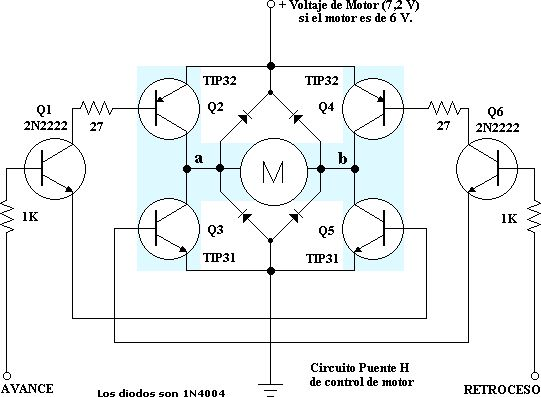
\includegraphics[width=0.45\textwidth]{IMAGENES/PuenteH_CIRCUITO_MARCOT.jpg}
        \caption{Circuito del puente H.}
        \label{fig:circuito_puenteh}
        \end{figure}

        Una de las principales ventajas del puente H es que permite invertir la polaridad aplicada a las terminales del motor sin necesidad de invertir físicamente las conexiones. Esto se consigue mediante la activación alternada de pares de transistores ubicados en las ramas diagonales del circuito.

    \subsection{El Transistor Bipolar (BJT) en Conmutación}
    Para comprender visualmente cómo opera el transistor en cada una de las distintas 
    regiones de operación, es útil compararlo analógicamente con el funcionamiento de un grifo de agua hidráulico:

    \begin{figure}[H]
        \centering
        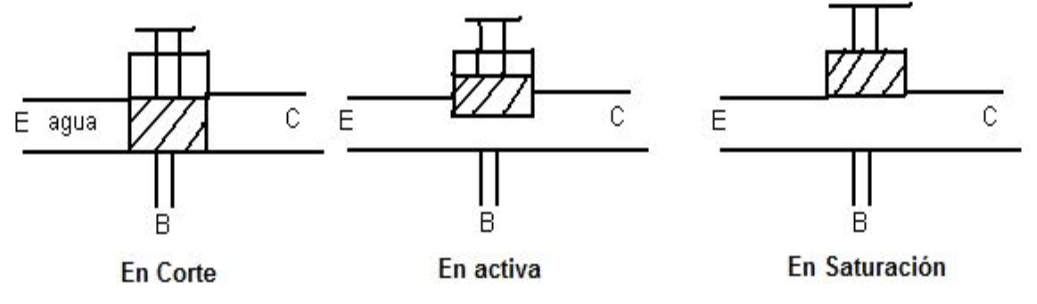
\includegraphics[width=0.45\textwidth]{IMAGENES/Estados_transistor.png}
        \caption{Analogía hidráulica de las tres regiones de operación del BJT.}
        \label{fig:estados_transitor}
    \end{figure}

    \subsubsection{Región de Corte (Grifo cerrado)}
    En este estado, la unión base-emisor no supera el umbral de conducción, por lo que no se inyecta corriente a la base ($I_B = 0$). 
    Al no existir un flujo de control que active el dispositivo, el transistor se comporta como un circuito abierto que impide el 
    paso de la corriente principal entre el colector y el emisor, idealmente provocando que $I_C = 0$.
    
    \subsubsection{Región Activa (Flujo controlado)}
    Es la zona de amplificación lineal del componente. Aquí, la apertura del canal es proporcional a la corriente inyectada en la terminal de control; 
    es decir, la corriente de colector ($I_C$) varía de forma lineal y proporcional a los cambios en la corriente de base ($I_B$). 
    
    Esta relación está gobernada por la ganancia de corriente de señal continua ($\beta$ o $h_{FE}$), modelada por la ecuación:
    \begin{equation}
        I_C = \beta \cdot I_B
        \label{ec:region_activa}
    \end{equation}

    \subsubsection{Región de Saturación (Grifo abierto al máximo)}
    En este punto, la corriente de base es lo suficientemente alta como para vencer la resistencia interna del silicio, provocando que ambas 
    uniones (base-emisor y colector-base) se polaricen en directo. Por más que se incremente el valor de $I_B$, 
    el flujo en el colector alcanza un límite máximo constante que ya no depende de la ganancia del semiconductor, 
    sino que está restringido exclusivamente por la fuente de alimentación ($V_{CC}$) y la resistencia de carga 
    del circuito ($R_L$). El transistor entra en saturación cuando se cumple la condición:

    \begin{equation}
        I_B > \frac{I_{C(\text{sat})}}{\beta_{\text{activa}}}
        \label{ec:condicion_sat}
    \end{equation}

    Bajo esta condición, la tensión entre colector y emisor cae a su valor mínimo posible, 
    denominado voltaje de saturación colector-emisor ($V_{CE(\text{sat})}$), 
    el cual representa la pérdida interna del componente en estado de conducción plena.

    \subsection{Redes de Conmutación y el Criterio de Saturación Forzada}
    Cuando el objetivo del diseño no es la amplificación lineal de señales, sino el control de dispositivos de potencia, 
    el BJT se configura para operar de forma binaria, alternando entre sus dos estados críticos: corte (bloqueo) y saturación (conducción). 
    En este modo de operación, el dispositivo prescinde de la región activa para comportarse como un interruptor de estado sólido ideal.
        
    Para garantizar un correcto desempeño del Puente H, el diseño debe asegurar que los transistores entren en una saturación profunda. 
    Esto se debe a que la ganancia de corriente real ($\beta$) de un transistor disminuye drásticamente a medida que el componente se 
    calienta o maneja corrientes elevadas en el colector. Si el transistor opera cerca del límite de la región activa, 
    el voltaje $V_{CE}$ aumentará, provocando severas pérdidas por disipación térmica:

    \begin{equation*}
        P_D = V_{CE(\text{sat})} \cdot I_C
        \label{ec:potencia_disipada}
    \end{equation*}

    Para blindar el circuito ante estas variaciones, la ingeniería de diseño aplica el criterio de Beta Forzada ($\beta_{\text{sat}}$). 
    Este método consiste en ignorar la $\beta$ nominal o de amplificación del datasheet y forzar un valor fijo, típicamente establecido en:

    \begin{equation*}
        \beta_{\text{forzada}} = 10
        \label{ec:beta_forzada}
    \end{equation*}

    Al diseñar las mallas limitadoras de base inyectando una corriente calculada como $I_B = I_C / 10$, se suministra un exceso controlado de portadores de carga a la base. Esto garantiza que, incluso bajo condiciones de máxima carga mecánica en el motor o fluctuaciones en el voltaje de alimentación, el transistor permanecerá firmemente en saturación, manteniendo el voltaje $V_{CE(\text{sat})}$ en su nivel mínimo y protegiendo al semiconductor de daños por sobrecalentamiento.
    
    \subsection{Cargas Inductivas y Elementos de Protección}
    El actuador electromecánico empleado en este circuito no se comporta como una carga puramente resistiva, sino como una carga inductiva compleja debido a los devanados de cobre que 
    constituyen su armadura interna. De acuerdo con la ley de inducción de Faraday, una bobina almacena 
    energía en forma de campo magnético mientras circula corriente a través de ella. 
    
    Sin embargo en el instante exacto en que los transistores del Puente H 
    conmutan del estado de saturación al de corte para detener o invertir el sentido de giro del motor, al interrumpirse abruptamente el flujo de corriente, el campo magnético 
    colapsa e induce una fuerza electromotriz (FEM) en forma de un transitorio de alta tensión inversa, dada por la ecuación diferencial:
    \begin{equation*}
        v_L(t) = L \frac{di(t)}{dt}
        \label{ec:fuerza_contraelectromotriz}
    \end{equation*}

    Este pico de voltaje puede superar severamente la tensión de ruptura colector-emisor ($V_{CEO}$) de los transistores, 
    destruyéndolos por avalancha térmica. Para mitigar este fenómeno, se integran \textbf{diodos de libre rueda} (\textit{flyback}) 
    en paralelo con cada BJT. Polarizados en inversa durante la operación normal, estos diodos entran en conducción directa ante el colapso magnético, 
    ofreciendo un camino seguro de baja impedancia para recircular la corriente residual. De este modo, se suprime el pico de alta tensión sujetando 
    el transitorio a la caída segura de la unión PN ($V_F \approx 0.7\text{ V}$), protegiendo la integridad de la etapa de potencia.

    \section{Materiales}
        \begin{figure} [H]
            \centering
            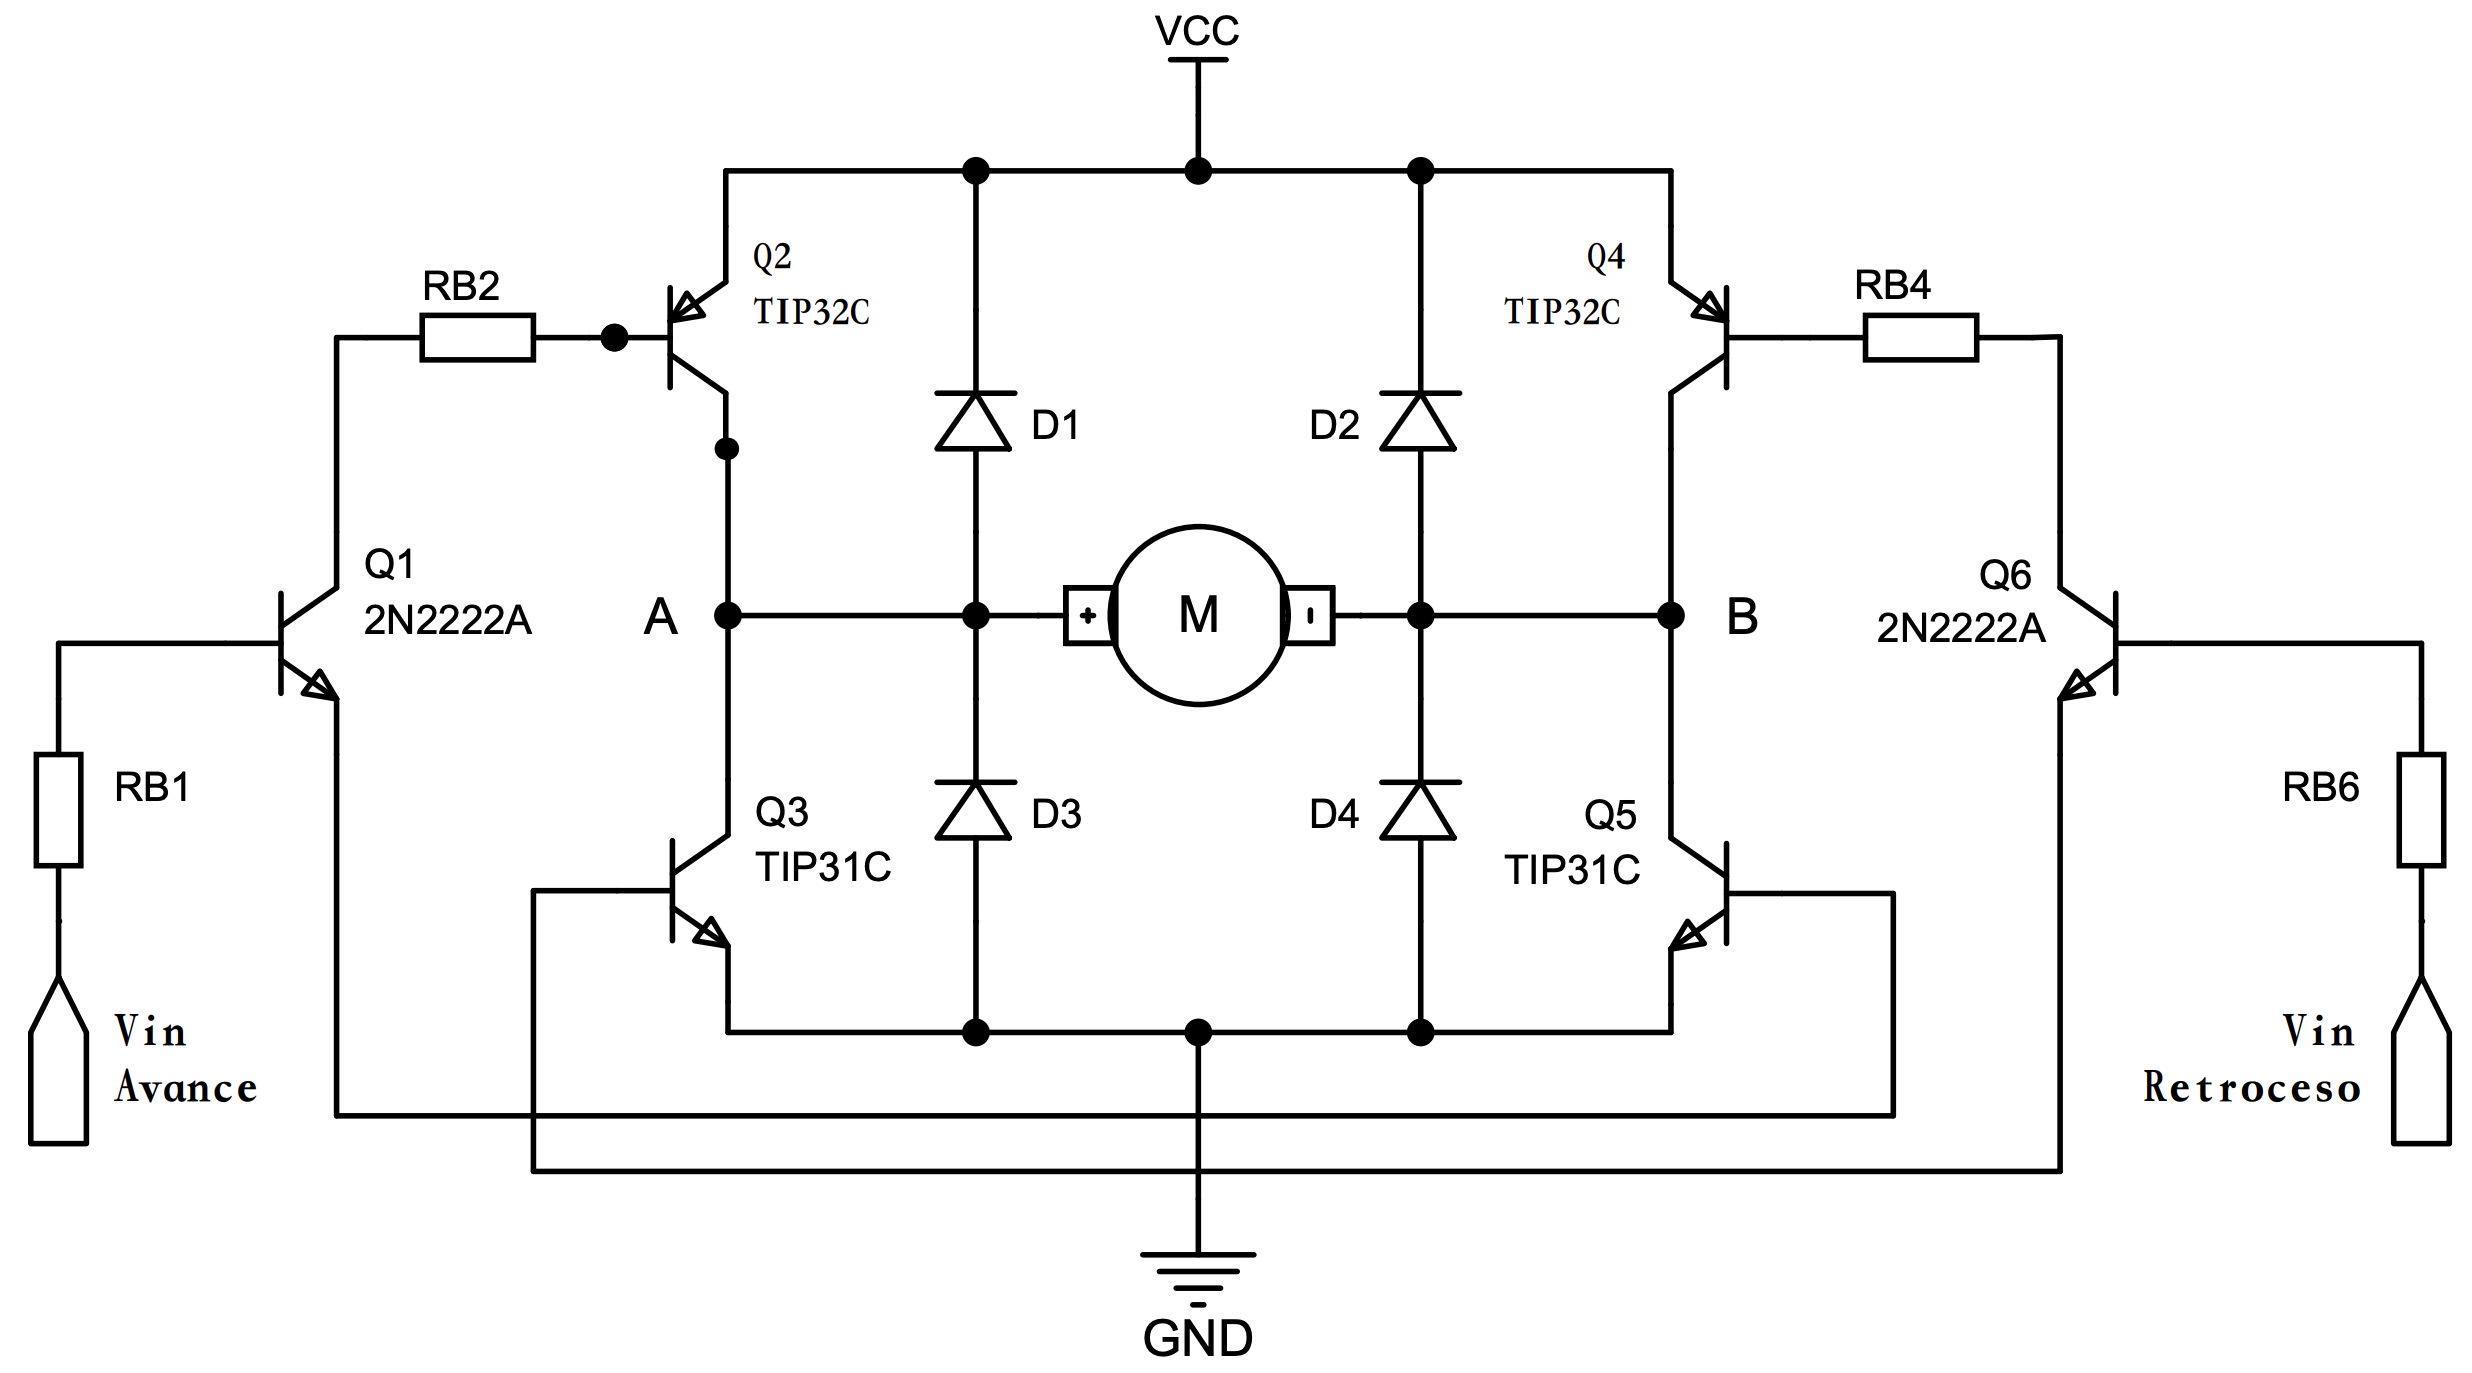
\includegraphics[width=0.48\textwidth]{IMAGENES/Circuito_PunteH.png}
            \caption{Circuito de un puente H.}
            \label{fig:Circuito_PunteH}
        \end{figure}
Para el circuito mostrado en la "Figura~\ref{fig:Circuito_PunteH}”, emplearemos:
    \begin{itemize}
        \item 2 transistores NPN 2N2222A
        \item 2 transistores TIP31C
        \item 2 transistores TIP32C
        \item 1 motor DC de 12 a 120mA
        \item 2 Resistencia de 330 $\Omega$ a 1/2W
        \item 2 Resistencia de 220 $\Omega$ a 1/2W
        \item 1 Protoboard
        \item 3 multímetros digitales (De preferencia)
        \item Cable para protoboard
    \end{itemize}

\section{Desarrollo}
    \subsection{Parámetros de diseño Puente H}
    Para facilitar el análisis se simplifico el circuito mostrado en la Figura \ref{fig:Circuito_PunteH} al analizar unicamente su comportamiento
    en la configuración de avance. Bajo estas condiciones los transistores Q4 y Q5 estarán en corte actuando como circuitos abiertos,
    por lo que es posible removerlos del diagrama. Asimismo, al sustituir la señal de control de avance y la línea de potencia $V_{CC}$ 
    por sus fuentes de alimentación equivalentes, se obtiene un circuito más sencillo compuesto por tres mallas como se muestra en la Figura \ref{fig:Circuito_simplificado}.
    
    \begin{figure} [H]
            \centering
            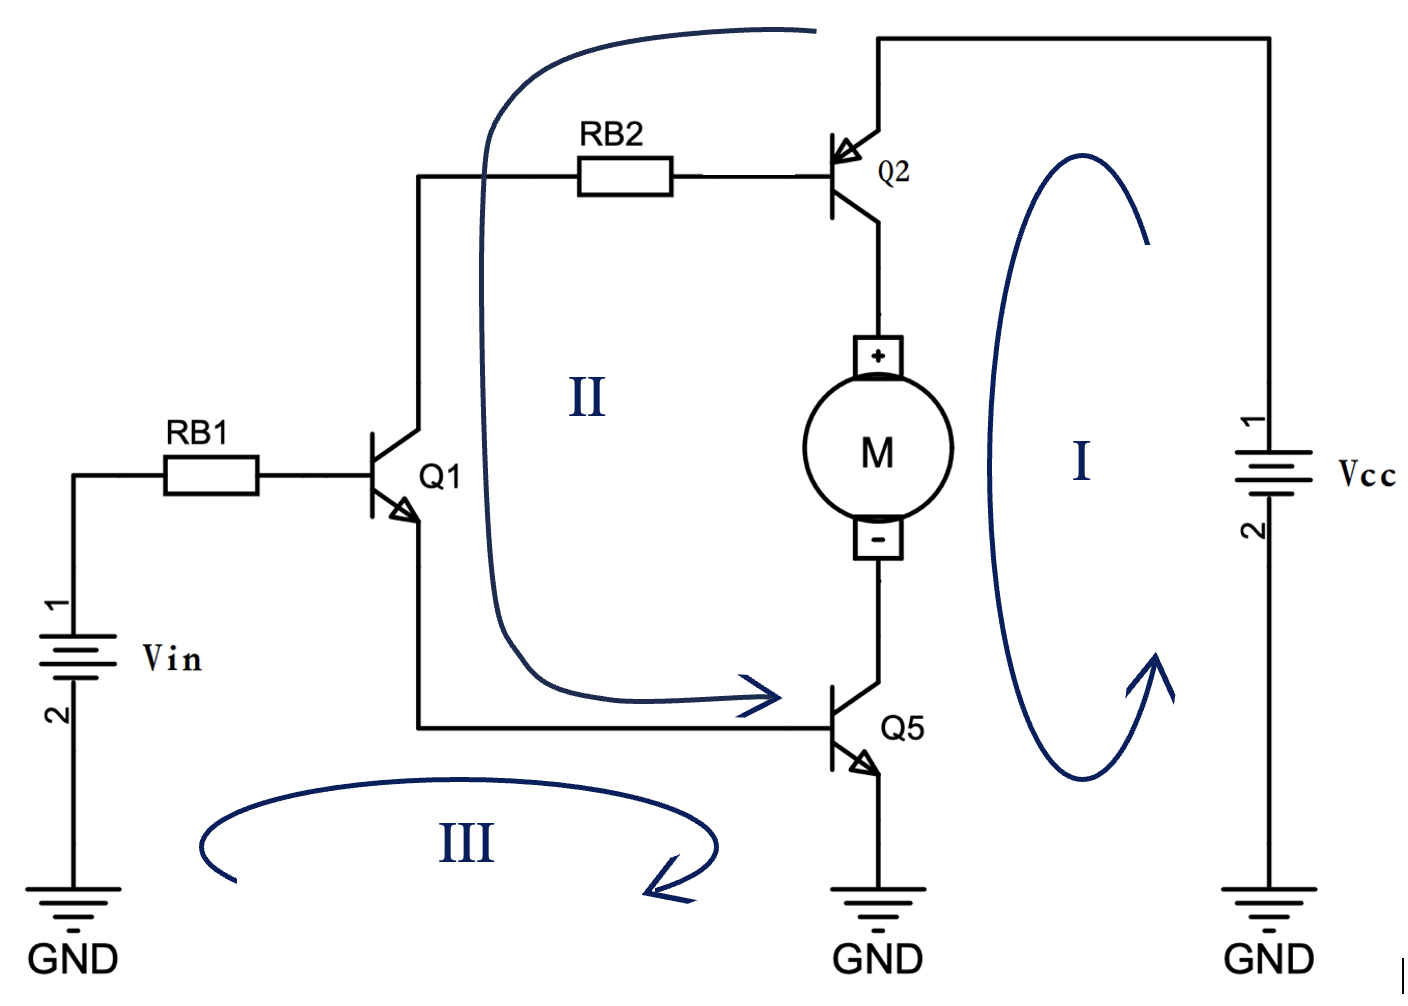
\includegraphics[width=0.48\textwidth]{IMAGENES/Mallas.png}
            \caption{Circuito simplificado.}
            \label{fig:Circuito_simplificado}
    \end{figure}
    
    Una vez denotada la polarización de voltajes y corrientes en el circuito, como se muestra en la Figura \ref{fig:Polarización_puenteH}, 
    se realizó el análisis de mallas siguiendo la convención de signos establecida. Cabe destacar que la dirección de las corrientes de 
    malla se determinó considerando la orientación física de las flechas en la simbología de los transistores, así como las condiciones 
    de polarización requeridas para activar y hacer girar el motor en el sentido deseado.
    
    \begin{figure} [H]
            \centering
            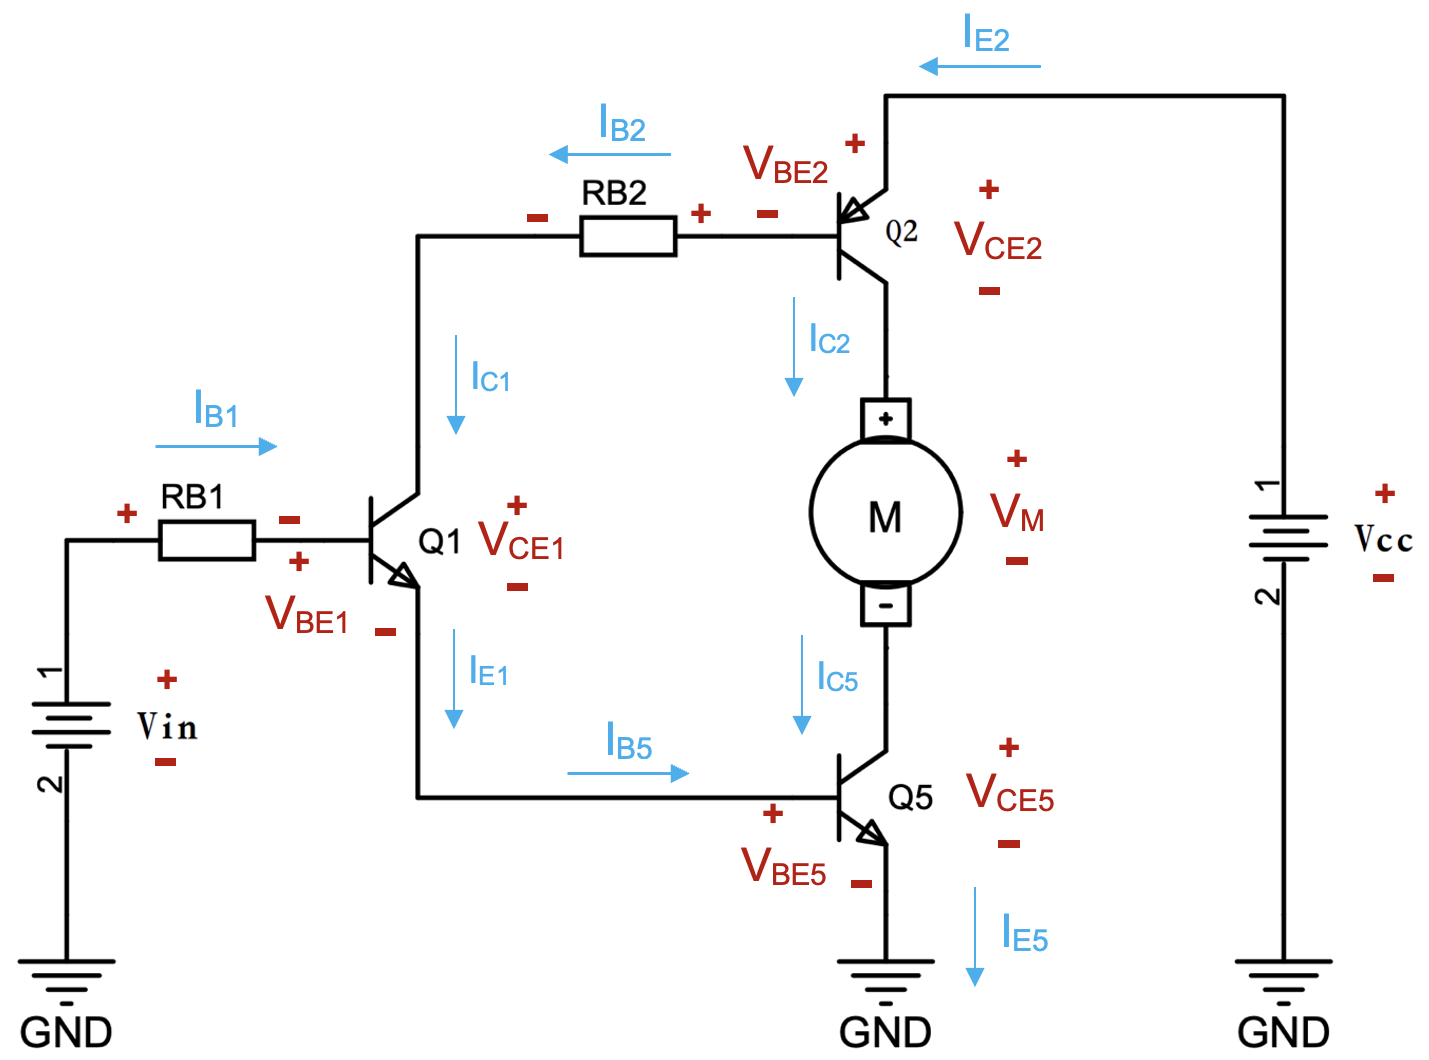
\includegraphics[width=0.48\textwidth]{IMAGENES/Circuito_simplificado.png}
            \caption{Polarización de transistor, resistores y fuentes en el circuito.}
            \label{fig:Polarización_puenteH}
    \end{figure}

    Para la primera malla, la ecuación de voltaje de Kirchhoff es: 
    \begin{equation}
        V_{CC} - V_{CE_{2}} - V_{M} - V_{CE_{5}} = 0
        \label{ec:Malla1}
    \end{equation}
    De manera similar, al analizar la segunda malla del circuito simplificado, se obtiene la siguiente expresión:
    \begin{equation}
        V_{CC} - V_{BE_{2}} - I_{B_{2}} R_{B_{2}} - V_{CE_{1}} - V_{BE_{5}} = 0
        \label{ec:Malla2}
    \end{equation}
    Finalmente analizando la malla de control 3 se obtiene un sistema de tres ecuaciones:
    \begin{equation}
        V_{in} - I_{B_{1}} R_{B_{1}} - V_{BE_{1}} - V_{BE_{5}} = 0
        \label{ec:Malla3}
    \end{equation}

    Donde se se obtiene un sistema de tres ecuaciones con dos incógnitas de diseño $R_{B_{2}}$ y $R_{B_{1}}$.

    A partir de las pruebas iniciales realizadas al motor, y bajo la condición de máxima carga aplicada, 
    se establecieron los parámetros de operación en $V_{\text{max}} = 10\text{ V}$ con una 
    corriente de $I_{\text{max}} = 200\text{ mA}$ para el actuador. 

    De igual modo se determinaron los parámetros correspondientes a cada transistor a partir 
    de las especificaciones técnicas de sus respectivas hojas de datos. Si tomamos en cuenta 
    que $I_M = I_{C2} = I_{C5}$ y una ganancia de saturación forzada $\beta = 10$, 
    se establece que:

    \begin{equation*}
        I_{B} = \frac{I_{C}}{\beta}
    \end{equation*}

    \begin{equation*}
        I_{B2} = \frac{I_{\text{max}}}{10} = \frac{200\text{ mA}}{10}
    \end{equation*}

    \begin{equation*}
        I_{B2} = 20\text{ mA}
    \end{equation*}

    Observando el esquema de la Figura \ref{fig:Circuito_simplificado} se nota que la corriente 
    de colector del transistor de control es suministrada por la base del transistor de potencia, 
    por lo tanto $I_{C1} = I_{B2}$. Empleando la misma relación analítica y proponiendo un valor 
    de $\beta = 10$ para asegurar la entrada en la región de saturación profunda del transistor 
    de pequeña señal, se obtiene: 

    \begin{equation*}
        I_{B1} = \frac{I_{C1}}{10} = \frac{20\text{ mA}}{10}
    \end{equation*}

    \begin{equation*}
        I_{B1} = 2\text{ mA}
    \end{equation*}

    Habiendo obtenido los valores de corriente de colector para cada uno de los transistores, 
    se extrajeron los parámetros de tensiones de saturación directamente de las curvas típicas 
    de los datasheets de los fabricantes (ver Anexo A) en base a la corriente máxima de 
    diseño $I_{\text{max}} = 200\text{ mA}$ y las corrientes de base previamente calculadas. 
    En la Tabla \ref{tab:voltajes_transistores} se presenta una recopilación limpia de estos 
    valores de diseño.

    \begin{table}[H]
    \centering
    \caption{Voltajes de operación de los transistores obtenidos de las hojas de datos y 
    valor de ganancia propuesto.}
    \label{tab:voltajes_transistores}
    \begin{tabular}{ccccc}
        \hline
        \textbf{Transistor} & \textbf{Modelo} & \textbf{$V_{BE}$ (V)} & \textbf{$V_{CE}$ (V)} & \textbf{Beta ($\beta$)} \\ \hline
        $Q_1, Q_6$          & 2N2222A         & 0.70                  & 0.10                  & 10                       \\ \hline
        $Q_2, Q_4$          & TIP32C          & 0.76                  & 0.10                  & 10                       \\ \hline
        $Q_3, Q_5$          & TIP31C          & 0.75                  & 0.05                  & 10                       \\ \hline
    \end{tabular}
    \end{table}

    Una vez recopilados los datos necesarios de las hojas de especificaciones de los transistores, 
    se procede a resolver el sistema de ecuaciones para determinar los valores comerciales de las 
    resistencias de base $R_{B1}$ y $R_{B2}$. 
    
    Para este análisis se establece un voltaje de alimentación de potencia $V_{CC} = 10\text{ V}$ y un voltaje de activación de entrada $V_{in} = 5\text{ V}$. 
    A partir de la ecuación \ref{ec:Malla1}, se calcula el voltaje real de operación que 
    recibe el actuador acoplado ($V_M$), en base a las caídas de tensión por saturación de 
    los transistores de potencia $Q_2$  y $Q_5$:

    \begin{equation*}
        V_{M} = V_{CC} - V_{CE_{2}} - V_{CE_{5}}
    \end{equation*}
    \begin{equation*}
        V_{M} = 10\text{ V} - 0.20\text{ V} - 0.05\text{ V} = 9.75\text{ V}
    \end{equation*}

    A continuación, se realiza el despeje de la resistencia de base $R_{B2}$ a partir de la ecuación de malla (\ref{ec:Malla2}). 
    \begin{equation*}
        V_{CC} - V_{BE_{2}} - I_{B_{2}} R_{B_{2}} - V_{CE_{1}} - V_{BE_{5}} = 0
    \end{equation*}

    \begin{equation*}
        R_{B2} = \frac{V_{CC} - V_{BE_{2}} - V_{CE_{1}} - V_{BE_{5}}}{I_{B_{2}}}
    \end{equation*}

    Sustituyendo los valores de tensión correspondientes y la corriente de base de 
    diseño $I_{B2} = 20\text{ mA}$ ($0.02\text{ A}$):

    \begin{equation*}
        R_{B2} = \frac{10\text{ V} - 0.76\text{ V} - 0.10\text{ V} - 0.75\text{ V}}{0.02\text{ A}}
    \end{equation*}

    \begin{equation*}
        R_{B2} = \frac{8.39\text{ V}}{0.02\text{ A}} = 419.5\text{ }\Omega
    \end{equation*}

    \begin{equation*}
        P_{R_{B2}} = 8.39\text{ V} (0.02\text{ A}) = 0.1678\text{ W}
    \end{equation*}

    Por lo tanto, se selecciona un valor comercial estándar de $430\text{ }\Omega$ a 1/2 W para $R_{B2}$.

    Finalmente, se analiza la malla de control de entrada (\ref{ec:Malla3}) para calcular la resistencia limitadora de base $R_{B1}$ del transistor 2N2222A, empleando la corriente calculada de $I_{B1} = 2\text{ mA}$ ($0.002\text{ A}$):

    \begin{equation*}
        V_{in} - I_{B_{1}} R_{B_{1}} - V_{BE_{1}} - V_{BE_{5}} = 0
    \end{equation*}

    \begin{equation*}
        R_{B1} = \frac{V_{in} - V_{BE_{1}} - V_{BE_{5}}}{I_{B_{1}}}
    \end{equation*}

    Sustituyendo los valores numéricos correspondientes:

    \begin{equation*}
        R_{B1} = \frac{5\text{ V} - 0.70\text{ V} - 0.75\text{ V}}{0.002\text{ A}}
    \end{equation*}

    \begin{equation*}
        R_{B1} = \frac{3.55\text{ V}}{0.002\text{ A}} = 1775\text{ }\Omega
    \end{equation*}

    \begin{equation*}
        P_{R_{B1}} = 3.55\text{ V} ( 0.002\text{ A} )= 0.0071\text{ W}
    \end{equation*}

    Igualmente se selecciona el valor comercial estándar más cercano, siendo este de $1.8\text{ k}\Omega$ a 1/2W.
    

    \subsection{Dimensionamiento de los Diodos}
    El análisis de protección se realiza bajo el escenario crítico de inversión de giro instantánea a máxima carga ($I_{\text{max}} = 200\text{ mA}$). 
    Debido a que la corriente en una inductancia no puede cambiar abruptamente, al pasar los transistores a corte, el campo magnético del motor 
    colapsa e induce una fuerza electromotriz (FEM) dada por $v_L(t) = L \, di/dt$. La corriente máxima acumulada 
    se transfiere íntegramente hacia la red de protección, estableciendo la corriente pico directa en:
    \begin{equation}
        I_{F_{\text{pico}}} = I_{\text{max}} = 200\text{ mA}
    \end{equation}

    Aplicando un factor de seguridad del 100\% ($FS = 2$) para prevenir sobrecorrientes por atasco mecánico, se determina el 
    requerimiento nominal continuo en $I_{F} = 400\text{ mA}$. 

    Por otro lado, la activación de los diodos sujeta el transitorio inductivo sumando el voltaje de 
    la fuente ($V_{CC} = 10\text{ V}$) y la caída de tensión directa del silicio ($V_F \approx 0.7\text{ V}$):
    \begin{equation*}
        V_{\text{transitorio}} = V_{CC} + V_{F}
    \end{equation*}
    \begin{equation*}
        V_{\text{transitorio}} = 10\text{ V} + 0.7\text{ V}
    \end{equation*}
    \begin{equation*}
        V_{\text{transitorio}} = 10.7\text{ V}
    \end{equation*}

    Bajo condiciones de bloqueo normal, los diodos en corte soportan directamente el voltaje de la fuente. Aplicando un factor de seguridad por picos en la línea, el voltaje inverso de ruptura repetitivo debe cumplir con $V_{RRM} \geq 20\text{ V}$. 

    Con base en estos límites ($I_F \geq 400\text{ mA}$, $V_{RRM} \geq 20\text{ V}$), se selecciona el diodo comercial \textbf{1N4001} ($1.0\text{ A}$, $50\text{ V}$ de operación máxima). Dado que los transistores TIP31C y TIP32C poseen un voltaje de ruptura colector-emisor de $V_{CEO} = 100\text{ V}$, el transitorio fijado a $10.7\text{ V}$ garantiza que los semiconductores operen firmemente dentro de su zona de trabajo segura.

    \subsection{Demostración de No Conducción en Estado de Avance}

    Para demostrar analíticamente que los diodos de protección permanecen inactivos (bloqueados) durante la operación normal en avance del motor, se analiza el estado de polarización de sus uniones PN.

    Cuando el Puente H se activa para el giro en avance, los transistores $Q_2$ (superior izquierdo, PNP) y $Q_5$ (inferior derecho, NPN) entran en saturación profunda. Esto provoca que el nodo del colector de $Q_2$ (conectado al ánodo del diodo superior $D_1$ y al cátodo del diodo inferior $D_3$) se eleve a un potencial casi igual al de la fuente:

    \begin{equation*}
        V_{A} = V_{CC} - V_{CE_{2}(\text{sat})}
    \end{equation*}
    \begin{equation*}
        V_{A} = 10\text{ V} - 0.20\text{ V}
    \end{equation*}
    \begin{equation*}
        V_{A} = 9.80\text{ V}
    \end{equation*}

    Simultáneamente, el colector de $Q_5$ (conectado al ánodo de $D_2$ y al cátodo de $D_4$) cae a un potencial de saturación mínimo respecto a tierra:

    \begin{equation}
        V_{B} = V_{CE_{5}(\text{sat})} = 0.05\text{ V}
    \end{equation}

    Analizando el estado de cada diodo bajo estas condiciones de voltaje:
    \begin{itemize}
        \item \textbf{Diodos Superiores ($D_1$ y $D_2$):} Sus cátodos están firmemente amarrados a $V_{CC} = 10\text{ V}$. Para $D_1$, el voltaje ánodo-cátodo es $V_{AK} = 9.80\text{ V} - 10\text{ V} = -0.20\text{ V}$. Al ser un valor negativo, el diodo experimenta una polarización inversa y se comporta como un circuito abierto.
        \item \textbf{Diodos Inferiores ($D_3$ y $D_4$):} Sus ánodos están conectados directamente a la referencia de tierra ($0\text{ V}$). Para $D_4$, el voltaje de la unión es $V_{AK} = 0\text{ V} - 0.05\text{ V} = -0.05\text{ V}$. De igual forma, al no superar el umbral de conducción del silicio ($V_{\gamma} \approx 0.7\text{ V}$), los diodos permanecen en estado de corte.
    \end{itemize}
    

\section{Análisis y Resultados}
    En la sección anterior se mostró de manera analítica, basándonos en las hojas de datos de cada uno de los componentes del circuito, los valores necesarios para trabajar en la región de saturación profunda y así garantizar el correcto funcionamiento del Puente H.
    Una vez obtenidos los valores de las resistencias de base y los diodos de protección, se procedió a la implementación del circuito en un protoboard para realizar las mediciones físicas de voltaje y corriente en cada uno de los transistores y el motor, obteniendo los siguientes valores en la Tabla \ref{tabla:Valores_medidos}.

    Algunas de las mediciones realizadas en laboratorio son las siguientes:

    \begin{table}[H]
    \centering
    \small 
    \begin{tabularx}{\columnwidth}{|c|X|X|}
    \hline
    \textbf{} & \textbf{2N2222A} & \textbf{TIP31C/TIP32C}\\ \hline
    $V_{BE}$  & 0.76V & 0.750V\\ \hline
    $V_{CE}$  & 0.20V & 25mV\\ \hline
    $I_B$ & 19.9mA & 120mA \\ \hline
    \end{tabularx}
    \caption{Voltajes y corrientes medidos}
    \label{tabla:Valores_medidos}
    \end{table}

    Conociendo estos valores es fácil deducir los valores de las betas de cada uno de los transistores; Partiendo de la siguiente ecuación:


        \[
        I_C = \beta I_B
        \]

        \[
        \beta = \frac{I_C}{I_B}
            = \frac{120\,\mathrm{mA}}{20\,\mathrm{mA}}
        \]

        \[
        \beta = 6
        \]

    \begin{table}[H]
    \centering
    \small 
    \begin{tabularx}{\columnwidth}{|c|X|X|X|X|}
    \hline
    \textbf{Transistor} & \textbf{Modelo} & \textbf{$\beta$ Datasheet} & \textbf{$\beta$ Calculado}\\ \hline
    $Q_1$, $Q_6$  & 2N2222A & 10 & 12\\ \hline
    $Q_2$, $Q_4$  & TIP32C &  10 & 6 \\ \hline
    $Q_3$, $Q_5$  & TIP31C &  10 & 6 \\ \hline

    \end{tabularx}
    \caption{Valores de $\beta$ calculados a partir de las mediciones}
    \label{tabla:Valores_beta}
    \end{table}

\section{Simulación}
    Para evaluar el comportamiento del circuito, se realizó una simulación en el software Multisim, la cual se ilustra a continuación:

    \begin{figure} [H]
            \centering
            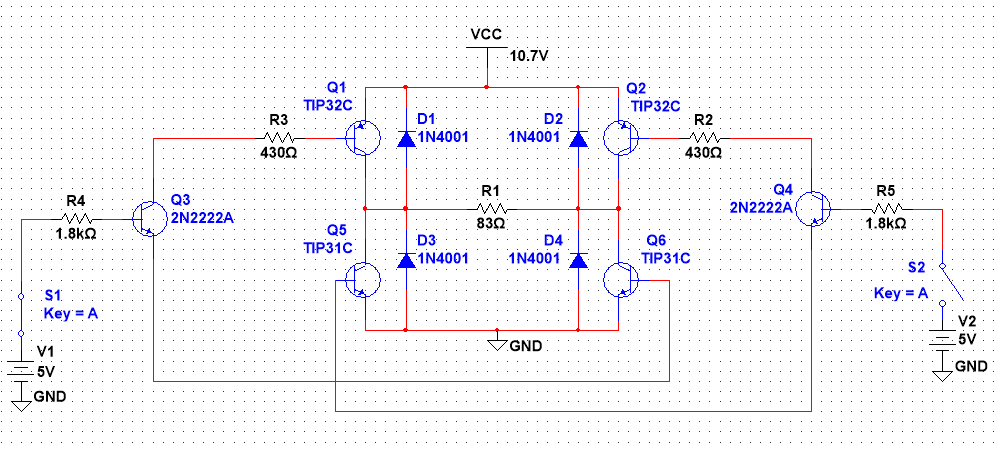
\includegraphics[width=0.48\textwidth]{IMAGENES/SIM.png}
            \caption{Circuito de puente H simulado con valores reales.}
            \label{fig:SIM1}
    \end{figure}

    Se utilizó una resistencia de 80 $\Omega$ para modelar las condiciones de máxima carga del motor empleado en el laboratorio. Cabe destactacar que estos valores mostrarán un resutado diferente al de las mediciones prácticas, debido a que el consumo de corriente real del motor varía dinámicamente en función de la carga mecánica aplicada.

    \begin{figure} [H]
            \centering
            
\includegraphics[width=0.48\textwidth]{IMAGENES/SIM1.png}
            \caption{Valores del motor simulado.}
            \label{fig:SIM_motor}
    \end{figure}

    La Tabla~\ref{tab:motor_comparativa} presenta la comparación inicial de los parámetros de voltaje y corriente en el elemento de carga.

    \begin{table}[H]
    \centering
    \caption{Comparación de voltajes y corrientes máximas en el motor.}
    \label{tab:motor_comparativa}
    \begin{tabular}{lcc}
        \hline
        \textbf{Valores} & \textbf{$V_{motor}$ (V)} & \textbf{$I_{motor}$ (mA)} \\ \hline
        Simulados        & 10.49                    & 131.23                    \\ \hline
        Medidos          & 10                       & 120                       \\ \hline
    \end{tabular}
    \end{table}

    \subsection{Medición y análisis de los transistores}

    A continuación, se examina el comportamiento operativo de cada transistor dentro del puente H, analizando las corrientes de base ($I_{base}$), colector ($I_{colector}$) y emisor ($I_{emisor}$) obtenidas en la simulación frente a las del laboratorio.

    En primer lugar, la Figura~\ref{fig:Valores_TIP32C} y la Tabla~\ref{tab:TIP32C_comparativa} muestran los resultados correspondientes al transistor de potencia PNP TIP32C.

    \begin{figure} [H]
            \centering
            
\includegraphics[width=0.48\textwidth]{IMAGENES/SIM2.png}
            \caption{Valores del TIP32C.}
            \label{fig:Valores_TIP32C}
    \end{figure}

    \begin{table}[H]
    \centering
    \caption{Comparación de corrientes en el TIP32C.}
    \label{tab:TIP32C_comparativa}
    \begin{tabular}{cccc}
        \hline
        \textbf{Valores} & \textbf{$I_{base}$ (mA)} & \textbf{$I_{colector}$ (mA)} & \textbf{$I_{emisor}$ (mA)} \\ \hline
        Simulados        & 21.374                   & 131.234                      & 152.609                    \\ \hline
        Medidos          & 10                       & 120                          & 120                        \\ \hline
    \end{tabular}
    \end{table}

    Posteriormente, se evalúa el comportamiento del transistor de potencia NPN TIP31C.

    \begin{figure} [H]
            \centering
            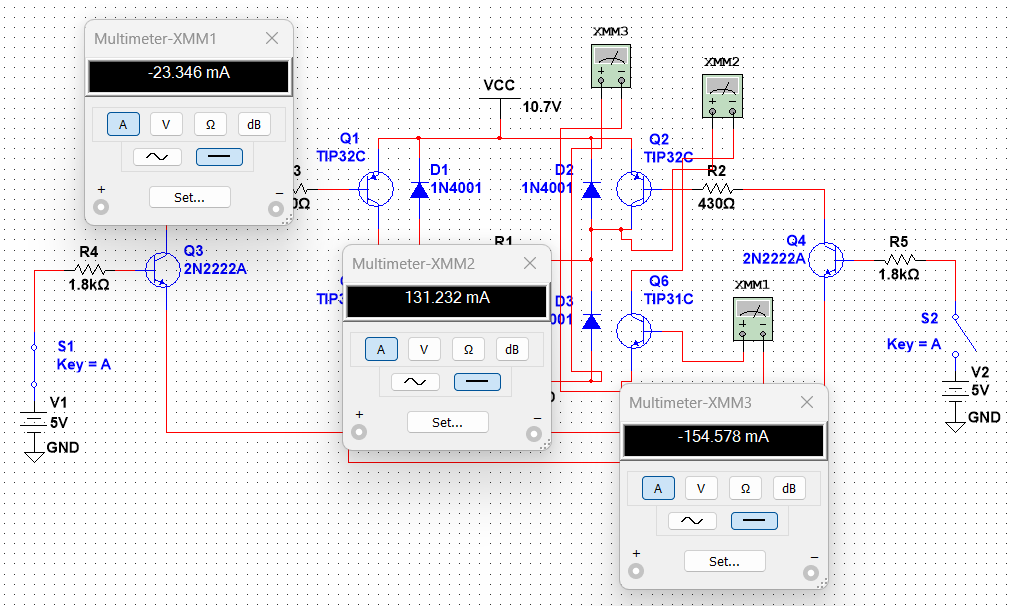
\includegraphics[width=0.48\textwidth]{IMAGENES/SIM3.png}
            \caption{Valores del TIP31C.}
            \label{fig:Valores_TIP31C}
    \end{figure}

    \begin{table}[H]
    \centering
    \caption{Comparación de corrientes en el TIP31C.}
    \label{tab:TIP31C_comparativa}
    \begin{tabular}{cccc}
        \hline
        \textbf{Valores} & \textbf{$I_{base}$ (mA)} & \textbf{$I_{colector}$ (mA)} & \textbf{$I_{emisor}$ (mA)} \\ \hline
        Simulados        & 23.346                   & 131.232                      & 154.578                    \\ \hline
        Medidos          & 10                       & 120                          & 120                        \\ \hline
    \end{tabular}
    \end{table}

    Finalmente, se presentan las condiciones de operación del transistor de control NPN 2N2222A.

    \begin{figure} [H]
            \centering
            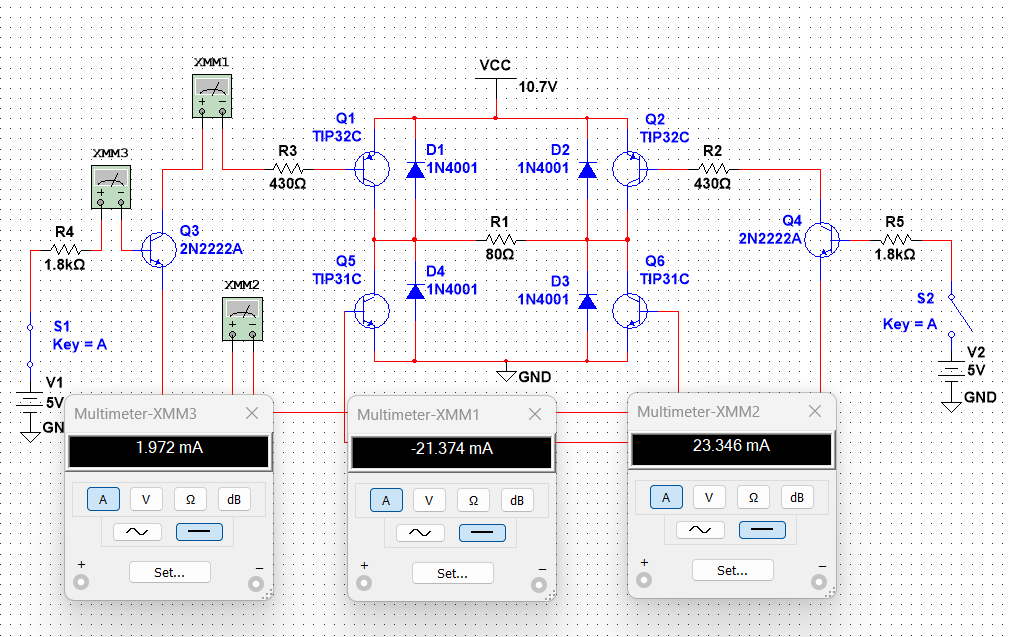
\includegraphics[width=0.48\textwidth]{IMAGENES/SIM4.png}
            \caption{Valores del 2N2222A.}
            \label{fig:Valores_2N2222A}
    \end{figure}

    \begin{table}[H]
    \centering
    \caption{Comparación de corrientes en el 2N2222A.}
    \label{tab:2N2222A_comparativa}
    \begin{tabular}{cccc}
        \hline
        \textbf{Valores} & \textbf{$I_{base}$ (mA)} & \textbf{$I_{colector}$ (mA)} & \textbf{$I_{emisor}$ (mA)} \\ \hline
        Simulados        & 1.972                    & 21.374                       & 23.346                     \\ \hline
        Medidos          & 10                       & 120                          & 120                        \\ \hline
    \end{tabular}
    \end{table}

    Los datos obtenidos mediante la simulación exhiben una consistencia teórica rigurosa. En primer lugar, se verifica el cumplimiento exacto de la Ley de Corrientes de Kirchhoff ($I_{emisor} = I_{base} + I_{colector}$) en cada uno de los componentes semiconductores. En segundo lugar, se observa un acoplamiento idóneo entre las etapas de control y de potencia: la corriente de colector del transistor driver 2N2222A ($21.374\text{ mA}$) suministra con precisión la corriente de activación requerida por la base del TIP32C, mientras que su corriente 
    de emisor ($23.346\text{ mA}$) comanda de forma directa la base del TIP31C. Este comportamiento ideal valida el diseño lógico del puente H y establece un marco de referencia sólido para el análisis de las desviaciones y efectos parásitos que se presenten en los datos experimentales.

\section{Conclusiones}
\begin{itemize}
    \item \textbf{Flores Cornejo Gustavo Mauricio.}
    \newline 
    La presente práctica sirvió para observar de manera práctica la contrucción y comportamiento dados ciertos parámetros del diseño de un puente H.A pesar, de que existen componentes que sustituyen
    o implementan de manefra más sencilla la funcionalidad del Puente H, es importante identificar la función de los transistores BJT así de la importancia de los diodos de protección en el circuito.
    Esdecir, esta práctica sirvió para implementar los temas vistos hasta el momento. Durante el desarrollo de esta práctica fue necesario ajustarnos a los valores reales del motor que conseguimos, por lo que
    tuvimos que rehacer y corrgeir en repetidas ocasiones los cálculos para aproximarnos de mejor manera a los valores reales de los componentes, además de que el esatdo de operación del motor fue utilizao bajo
    un torque alto, aumentando así la corriente de operación del motor y alterando de igual manera los valores reales del circuito.
    También fue interesante observar y analizar el comportamiento del transistor en su estado de saturación.
    \newline 
    \item \textbf{Muñoz Reyes Arturo Yabet.}
    \newline Esta práctica nos deja en claro la función de los transistores bipolares (TIP32C, TIP31C y los excitadores 2N2222A) en la aplicación para un puente H los cuales actúan como interruptores electrónicos de estado sólido. Podemos obsevar que al recibir una señal de control en sus respectivas bases, estos semiconductores operan entre sus regiones de corte y saturación. Permitiendo habilitar pares diagonales específicos de transistores para conmutar la polaridad de la fuente principal de 10.7V sobre la carga central (R1), controlando así la dirección del flujo de corriente y el sentido del giro del motor.
    Cabe destacar que determinar matemáticamente las mallas de entrada, las ganancias (Beta) y las corrientes de base necesarias permite dimensionar correctamente las resistencias limitadoras (R2, R3, R4, R5). La práctica nos deja ver que estos cálculos son fundamentales para garantizar que los transistores alcancen una saturación profunda, minimizando la disipación de calor y las caídas de tensión no deseadas, asegurando así un diseño eficiente y seguro antes de su implementación física.
    \item \textbf{Morales Vásquez Miguel Ehecatl.} 
    \newline Esta práctica permitió comprender de manera integral el diseño, la construcción y el comportamiento dinámico de un puente H discreto, conectando los fundamentos teóricos del transistor BJT con su aplicación física. Aunque existen circuitos integrados que simplifican esta función, la implementación con transistores discretos (TIP31C, TIP32C y excitadores 2N2222A) permitió analizar su operación como interruptores de estado sólido, operando entre corte y saturación para alternar la polaridad de la fuente sobre la carga y controlar la dirección del motor. El análisis matemático de las mallas, la ganancia ($\beta$) y las corrientes de base resultó indispensable para dimensionar las resistencias limitadoras y garantizar una saturación profunda que minimice la disipación de calor y las pérdidas de tensión. Además, el trabajo experimental bajo alto torque incrementó la corriente consumida, lo que exigió recalibrar los cálculos teóricos frente a las condiciones reales del motor y constatar el papel esencial de los diodos de protección para absorber las sobretensiones inductivas de la carga.
    
\end{itemize}



% if have a single appendix:
%\appendix[Proof of the Zonklar Equations]
% or
%\appendix  % for no appendix heading
% do not use \section anymore after \appendix, only \section*
% is possibly needed

% use appendices with more than one appendix
% then use \section to start each appendix
% you must declare a \section before using any
% \subsection or using \label (\appendices by itself
% starts a section numbered zero.)

\appendices
\section{Datasheets}

    \begin{figure}[H]
    \centering
    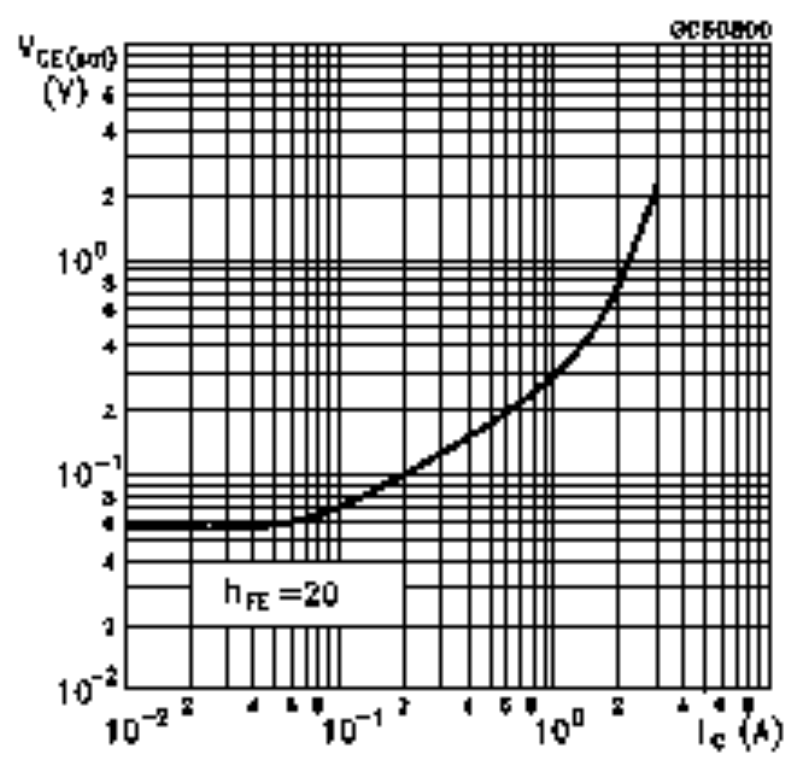
\includegraphics[width=0.37\textwidth]{IMAGENES/CollectorEmitter_saturation_Tip32C.png} 
    \caption{Collector emitter saturation voltage, Tip32C.}
    \label{fig:CollectorEmitter_Tip32C}
    \end{figure}

    \begin{figure}[H]
    \centering
    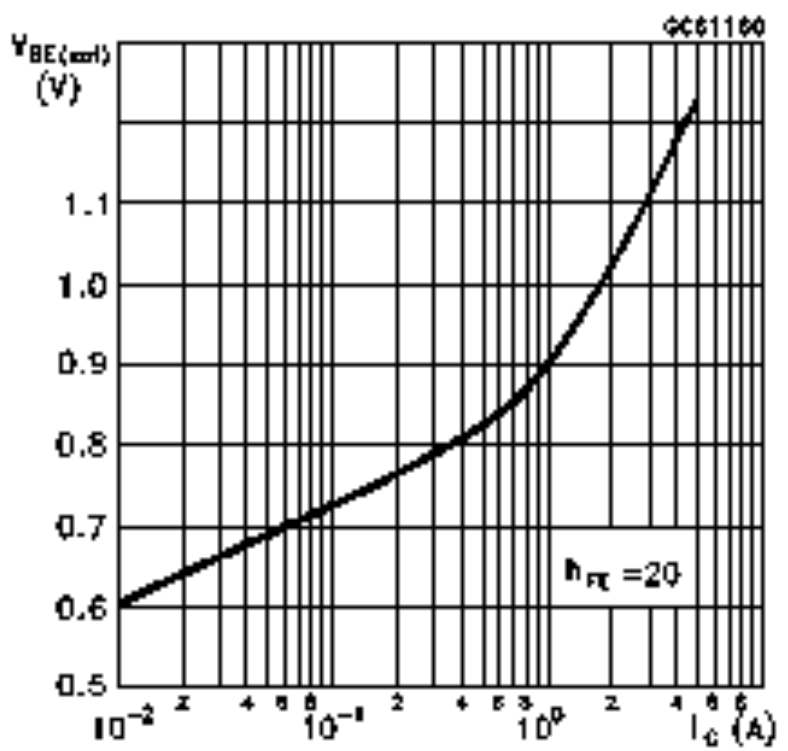
\includegraphics[width=0.37\textwidth]{IMAGENES/BaseEmitter_saturation_Tip32C.png} 
    \caption{Base emitter saturation voltage, Tip32C.}
    \label{fig:BaseEmitter_Tip32C}
    \end{figure}

    \begin{figure}[H]
    \centering
    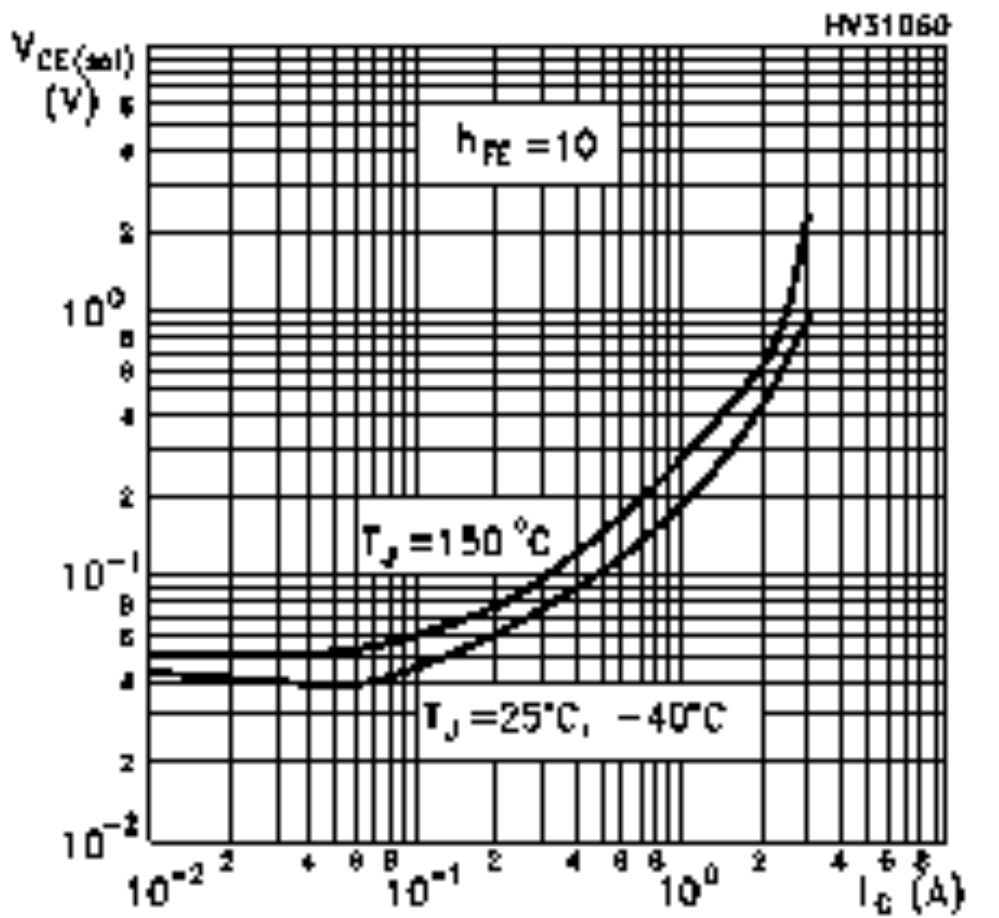
\includegraphics[width=0.37\textwidth]{IMAGENES/CollectorEmitter_saturation_Tip31C.png} 
    \caption{Collector emitter saturation voltage, Tip31C.}
    \label{fig:CollectorEmitter_Tip31C}
    \end{figure}

    \begin{figure}[H]
    \centering
    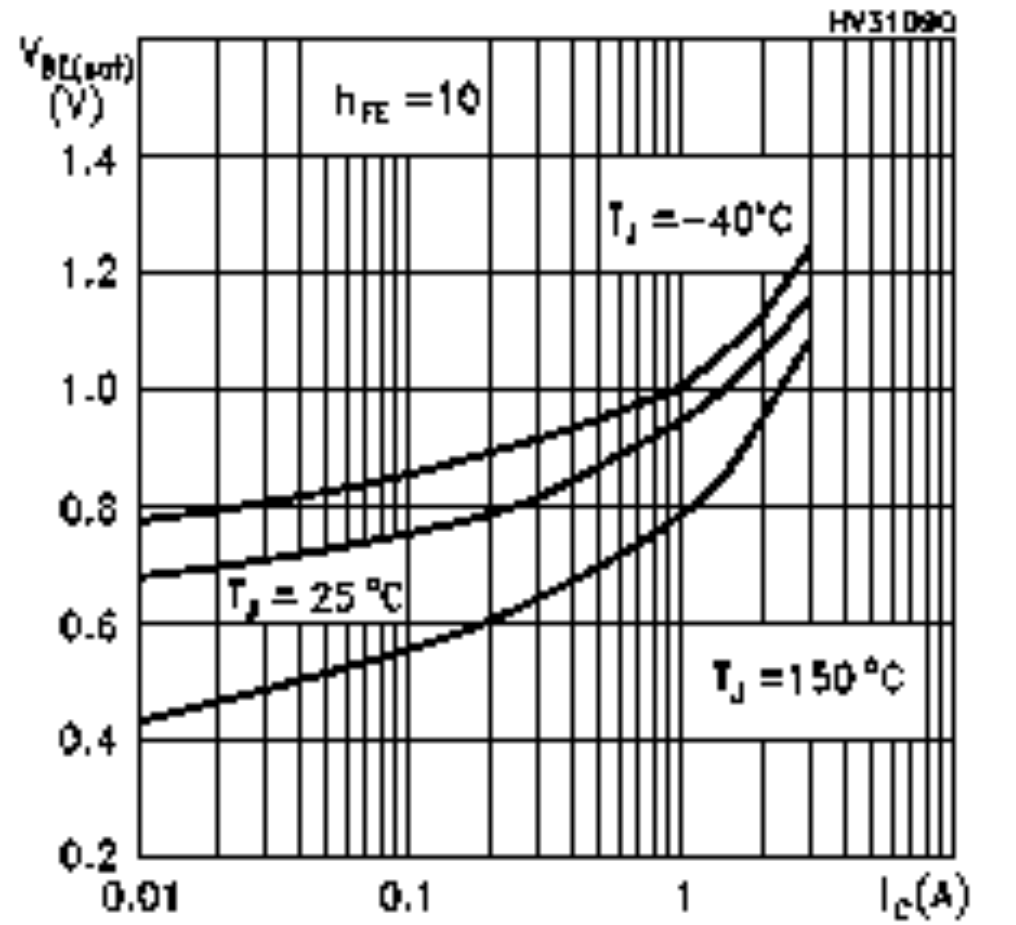
\includegraphics[width=0.37\textwidth]{IMAGENES/BaseEmitter_saturation_Tip31C.png} 
    \caption{Base emitter saturation voltage, Tip31C.}
    \label{fig:BaseEmitter_Tip31C}
    \end{figure}

    \begin{figure}[H]
    \centering
    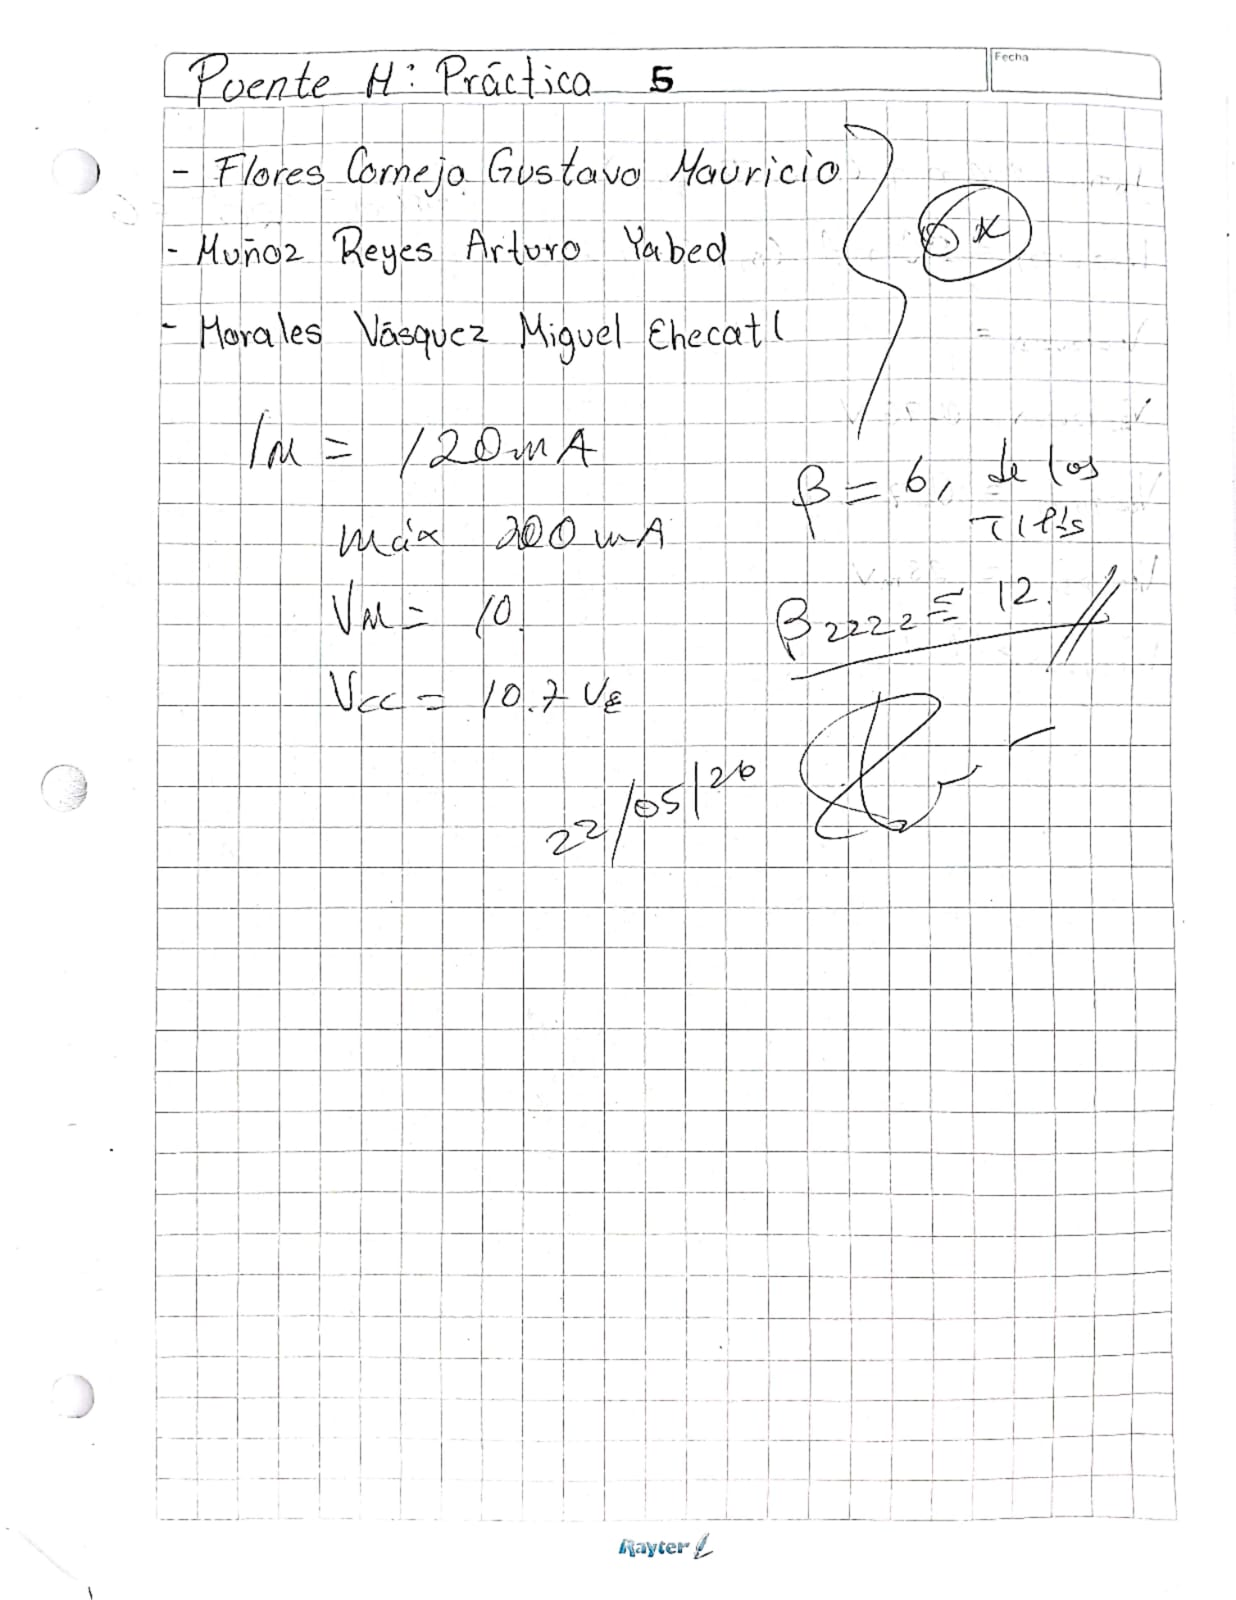
\includegraphics[width=0.37\textwidth]{IMAGENES/PuenteH_Firma.jpeg} 
    \caption{Evidencia de elaboración de práctica en laboratorio.}
    \label{fig:Firma_PuenteH}
    \end{figure}
  

\begin{thebibliography}{100}

    \bibitem{boylestad}
    R. L. Boylestad and L. Nashelsky, \textit{Electronic Devices and Circuit Theory}, 
    10th ed. Upper Saddle River, NJ, USA: Prentice Hall, 2009.

    \bibitem{datasheetTIP}
    STMicroelectronics, ``TIP31C, TIP32C: Complementary power transistors,'' \textit{TIP32C Datasheet}, 
    DocID4136 Rev 7, Jul. 2014. [Online]. Available: 
    https://www.alldatasheet.com/html-pdf/556838/STMICROELECTRONICS/TIP32C/7790/4/TIP32C.html. [Accessed: Jun. 11, 2026].

\end{thebibliography}


% that's all folks
\end{document}